% Options for packages loaded elsewhere
\PassOptionsToPackage{unicode}{hyperref}
\PassOptionsToPackage{hyphens}{url}
\PassOptionsToPackage{dvipsnames,svgnames,x11names}{xcolor}
%
\documentclass[
  11pt,
  letterpaper]{article}
\usepackage{amsmath,amssymb}
\usepackage{iftex}
\ifPDFTeX
  \usepackage[T1]{fontenc}
  \usepackage[utf8]{inputenc}
  \usepackage{textcomp} % provide euro and other symbols
\else % if luatex or xetex
  \usepackage{unicode-math} % this also loads fontspec
  \defaultfontfeatures{Scale=MatchLowercase}
  \defaultfontfeatures[\rmfamily]{Ligatures=TeX,Scale=1}
\fi
\usepackage{lmodern}
\ifPDFTeX\else
  % xetex/luatex font selection
\fi
% Use upquote if available, for straight quotes in verbatim environments
\IfFileExists{upquote.sty}{\usepackage{upquote}}{}
\IfFileExists{microtype.sty}{% use microtype if available
  \usepackage[]{microtype}
  \UseMicrotypeSet[protrusion]{basicmath} % disable protrusion for tt fonts
}{}
\makeatletter
\@ifundefined{KOMAClassName}{% if non-KOMA class
  \IfFileExists{parskip.sty}{%
    \usepackage{parskip}
  }{% else
    \setlength{\parindent}{0pt}
    \setlength{\parskip}{6pt plus 2pt minus 1pt}}
}{% if KOMA class
  \KOMAoptions{parskip=half}}
\makeatother
\usepackage{xcolor}
\usepackage[margin=1in]{geometry}
\usepackage{color}
\usepackage{fancyvrb}
\newcommand{\VerbBar}{|}
\newcommand{\VERB}{\Verb[commandchars=\\\{\}]}
\DefineVerbatimEnvironment{Highlighting}{Verbatim}{commandchars=\\\{\}}
% Add ',fontsize=\small' for more characters per line
\usepackage{framed}
\definecolor{shadecolor}{RGB}{248,248,248}
\newenvironment{Shaded}{\begin{snugshade}}{\end{snugshade}}
\newcommand{\AlertTok}[1]{\textcolor[rgb]{0.94,0.16,0.16}{#1}}
\newcommand{\AnnotationTok}[1]{\textcolor[rgb]{0.56,0.35,0.01}{\textbf{\textit{#1}}}}
\newcommand{\AttributeTok}[1]{\textcolor[rgb]{0.13,0.29,0.53}{#1}}
\newcommand{\BaseNTok}[1]{\textcolor[rgb]{0.00,0.00,0.81}{#1}}
\newcommand{\BuiltInTok}[1]{#1}
\newcommand{\CharTok}[1]{\textcolor[rgb]{0.31,0.60,0.02}{#1}}
\newcommand{\CommentTok}[1]{\textcolor[rgb]{0.56,0.35,0.01}{\textit{#1}}}
\newcommand{\CommentVarTok}[1]{\textcolor[rgb]{0.56,0.35,0.01}{\textbf{\textit{#1}}}}
\newcommand{\ConstantTok}[1]{\textcolor[rgb]{0.56,0.35,0.01}{#1}}
\newcommand{\ControlFlowTok}[1]{\textcolor[rgb]{0.13,0.29,0.53}{\textbf{#1}}}
\newcommand{\DataTypeTok}[1]{\textcolor[rgb]{0.13,0.29,0.53}{#1}}
\newcommand{\DecValTok}[1]{\textcolor[rgb]{0.00,0.00,0.81}{#1}}
\newcommand{\DocumentationTok}[1]{\textcolor[rgb]{0.56,0.35,0.01}{\textbf{\textit{#1}}}}
\newcommand{\ErrorTok}[1]{\textcolor[rgb]{0.64,0.00,0.00}{\textbf{#1}}}
\newcommand{\ExtensionTok}[1]{#1}
\newcommand{\FloatTok}[1]{\textcolor[rgb]{0.00,0.00,0.81}{#1}}
\newcommand{\FunctionTok}[1]{\textcolor[rgb]{0.13,0.29,0.53}{\textbf{#1}}}
\newcommand{\ImportTok}[1]{#1}
\newcommand{\InformationTok}[1]{\textcolor[rgb]{0.56,0.35,0.01}{\textbf{\textit{#1}}}}
\newcommand{\KeywordTok}[1]{\textcolor[rgb]{0.13,0.29,0.53}{\textbf{#1}}}
\newcommand{\NormalTok}[1]{#1}
\newcommand{\OperatorTok}[1]{\textcolor[rgb]{0.81,0.36,0.00}{\textbf{#1}}}
\newcommand{\OtherTok}[1]{\textcolor[rgb]{0.56,0.35,0.01}{#1}}
\newcommand{\PreprocessorTok}[1]{\textcolor[rgb]{0.56,0.35,0.01}{\textit{#1}}}
\newcommand{\RegionMarkerTok}[1]{#1}
\newcommand{\SpecialCharTok}[1]{\textcolor[rgb]{0.81,0.36,0.00}{\textbf{#1}}}
\newcommand{\SpecialStringTok}[1]{\textcolor[rgb]{0.31,0.60,0.02}{#1}}
\newcommand{\StringTok}[1]{\textcolor[rgb]{0.31,0.60,0.02}{#1}}
\newcommand{\VariableTok}[1]{\textcolor[rgb]{0.00,0.00,0.00}{#1}}
\newcommand{\VerbatimStringTok}[1]{\textcolor[rgb]{0.31,0.60,0.02}{#1}}
\newcommand{\WarningTok}[1]{\textcolor[rgb]{0.56,0.35,0.01}{\textbf{\textit{#1}}}}
\usepackage{graphicx}
\makeatletter
\newsavebox\pandoc@box
\newcommand*\pandocbounded[1]{% scales image to fit in text height/width
  \sbox\pandoc@box{#1}%
  \Gscale@div\@tempa{\textheight}{\dimexpr\ht\pandoc@box+\dp\pandoc@box\relax}%
  \Gscale@div\@tempb{\linewidth}{\wd\pandoc@box}%
  \ifdim\@tempb\p@<\@tempa\p@\let\@tempa\@tempb\fi% select the smaller of both
  \ifdim\@tempa\p@<\p@\scalebox{\@tempa}{\usebox\pandoc@box}%
  \else\usebox{\pandoc@box}%
  \fi%
}
% Set default figure placement to htbp
\def\fps@figure{htbp}
\makeatother
\setlength{\emergencystretch}{3em} % prevent overfull lines
\providecommand{\tightlist}{%
  \setlength{\itemsep}{0pt}\setlength{\parskip}{0pt}}
\setcounter{secnumdepth}{-\maxdimen} % remove section numbering
\usepackage[notextcomp]{kpfonts}
\usepackage{Inconsolata}
\usepackage{caption}
\usepackage{float}
\captionsetup*{labelfont={sc},textfont={it},labelsep={colon},justification=centering,singlelinecheck=true}
\usepackage{bookmark}
\IfFileExists{xurl.sty}{\usepackage{xurl}}{} % add URL line breaks if available
\urlstyle{same}
\hypersetup{
  pdfauthor={John Koo},
  pdfsubject={Week 1 Handout},
  colorlinks=true,
  linkcolor={Maroon},
  filecolor={Maroon},
  citecolor={Blue},
  urlcolor={blue},
  pdfcreator={LaTeX via pandoc}}

\title{\textsc{Week 1 Handout}}
\usepackage{etoolbox}
\makeatletter
\providecommand{\subtitle}[1]{% add subtitle to \maketitle
  \apptocmd{\@title}{\par {\large #1 \par}}{}{}
}
\makeatother
\subtitle{Gov 50 Data Science for Social Sciences}
\author{John Koo}
\date{September 2, 2025}

\begin{document}
\maketitle

\section{Contact Info}\label{contact-info}

\begin{table}[!h]

\centering

\begin{tabular}{l}
  \textbf{John Koo} \\
  PhD Candidate, Department of Government \\ \\
  
  \textbf{Email} (preferred): \href{mailto:johnkoo@fas.harvard.edu}{johnkoo@fas.harvard.edu} \\
  \textbf{Slack}: @johnkoo (in the Harvard University workspace) \\
  \textbf{Office hours}: Tuesdays, 1:30pm to 3:30pm @ CGIS Cafe (sign-up: \href{https://jkoo.nl/meet}{jkoo.nl/meet}) \\ \\ 
  \textbf{Section materials}: \url{https://github.com/tanxpyox/gov50-sections-jk}
  
  \end{tabular}
\end{table}

\section{Where to get help?}\label{where-to-get-help}

\begin{itemize}
\item
  For tech assistance or help with homework: \textbf{Course
  Assistant-led Study Halls}

  \begin{quote}
  Study halls are a combination of office hours and drop-in tutoring
  sessions. Course assistants will hold a table usually at one of the
  house dining halls or common rooms and help students with assignments
  and course material. Study halls work best if you come as a group and
  work on the assignments on your own while you are there and ask for
  help from the CAs when you get stuck.
  \end{quote}

  \begin{quote}
  Schedule: Mondays and Wednesdays, 5pm to 9pm (see Syllabus for
  location)
  \end{quote}
\item
  For initial help with course content: ask on course Slack (accessible
  via Canvas sidebar) or sign up for my office hours
\item
  For perspective and inspiration: sign up for Scott's office hours
\end{itemize}

\section{Getting the most (grades) out of this
class}\label{getting-the-most-grades-out-of-this-class}

\begin{itemize}
\tightlist
\item
  Podcast and Article Responses (5\%) {[}one two-page doc every other
  week{]}
\item
  Problem Sets (20\%) {[}seven to eight in total{]}
\item
  Mid-term exam (20\%) {[}in-class, written, closed book{]}
\item
  Final exam (20\%) {[}in-class, written, closed book{]}
\item
  \emph{Final project} (25\%)
\end{itemize}

\newpage

Generic advice for maximising grades and efficiency

\begin{itemize}
\tightlist
\item
  Everything you learn should help you work towards the final project
  (which is the biggest chunk of your grades)

  \begin{itemize}
  \tightlist
  \item
    Take the project milestones seriously and do not wait until the last
    minute
  \end{itemize}
\item
  Problem sets

  \begin{itemize}
  \tightlist
  \item
    Low hanging fruits - don't miss them; Can reuse code in your
    projects
  \item
    It's OK to make mistakes (each p-set is 2--3\% of your final grade)
  \item
    Work with your study group; but write up your p-sets individually
  \item
    Start early, so you have time to get help
  \item
    Set aside a ``focus session'' every week to do the problem sets; do
    not mull over the p-set for the whole week
  \end{itemize}
\item
  AI allowed and encouraged, except in exams. Start learning how to use
  AI to debug your code.
\item
  Keep your code organised in your GitHub repository - you may need them
  in your final project
\end{itemize}

\section{Getting Started}\label{getting-started}

\begin{itemize}
\item
  Software: R, RStudio
\item
  Version control: Git and GitHub
\end{itemize}

\begin{figure}
\centering
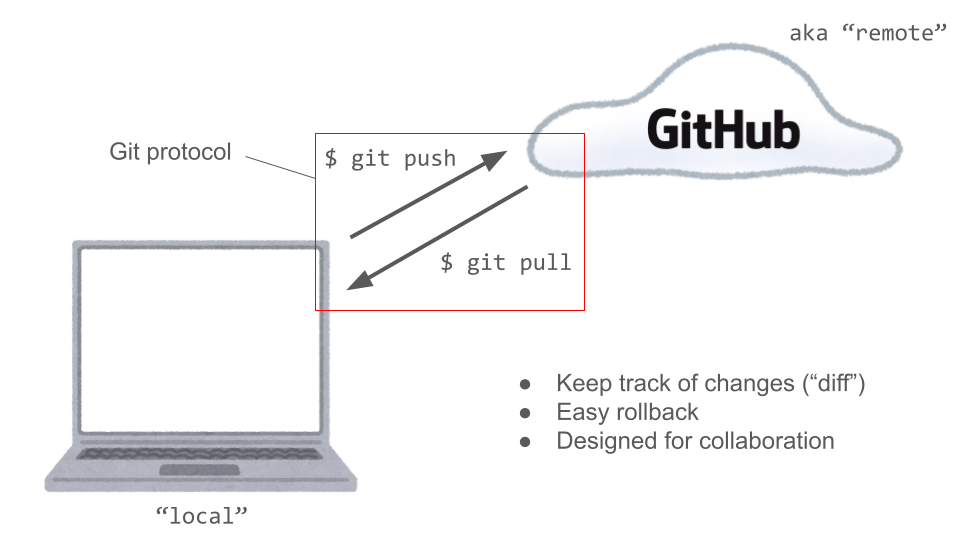
\includegraphics[width=0.75\linewidth,height=\textheight,keepaspectratio]{assets/gitvsgithub.png}
\caption{Git and GitHub}
\end{figure}

\newpage

\begin{center}
  \section{Problem Set 0a: GitHub Setup}
  \textbf{Due: Wednesday, September 10, 2024 at 11:59 PM}
\end{center}

\subsection{Overview}\label{overview}

This assignment will get you set up with GitHub, which we'll use
throughout the semester to share code and track your work. Think of
GitHub as Google Docs for code - it saves your history and lets you
collaborate.

\subsection{What You'll Do}\label{what-youll-do}

\begin{enumerate}
\def\labelenumi{\arabic{enumi}.}
\tightlist
\item
  Create a GitHub account
\item
  Create your first repository
\item
  Edit a \texttt{README} file
\item
  Submit proof to Gradescope
\end{enumerate}

\subsection{Step-by-Step Instructions}\label{step-by-step-instructions}

\subsubsection{Part 1: Create Your GitHub
Account}\label{part-1-create-your-github-account}

\begin{enumerate}
\def\labelenumi{\arabic{enumi}.}
\tightlist
\item
  Go to \url{https://github.com}
\item
  Click ``Sign up''
\item
  Choose a username (this will be public, so pick something
  professional)
\item
  Use your Harvard email (optional)
\item
  Complete the signup process
\item
  Download GitHub Desktop and log in with your new account
\end{enumerate}

\subsubsection{Part 2: Create Your First
Repository}\label{part-2-create-your-first-repository}

\begin{enumerate}
\def\labelenumi{\arabic{enumi}.}
\tightlist
\item
  On GitHub Desktop, click ``Add'' \textgreater{} ``Create New
  Repository''
\item
  Name the repository \texttt{gov50-fall2024}
\item
  Set the local path to a folder where you'll keep your course work
\item
  Choose ``R'' as the language
\item
  Click ``Create Repository''
\item
  Click ``Publish repository'' to upload it to GitHub (make sure ``Keep
  this code private'' is checked; you will be make a public repo later
  for your projects)
\end{enumerate}

\subsubsection{Part 3: Set up RStudio}\label{part-3-set-up-rstudio}

\begin{enumerate}
\def\labelenumi{\arabic{enumi}.}
\tightlist
\item
  Open RStudio
\item
  Go to ``File'' \textgreater{} ``New Project'' \textgreater{}
  ``Existing Directory'' \textgreater{} Choose the GitHub folder you
  just created
\item
  Click ``Create Project''
\item
  Click ``New File'', name it as \texttt{README.md}, and save it in the
  project directory
\end{enumerate}

\subsubsection{Part 4: Edit Your README}\label{part-4-edit-your-readme}

\begin{enumerate}
\def\labelenumi{\arabic{enumi}.}
\tightlist
\item
  Click on the \texttt{README.md} file
\item
  Add:
\end{enumerate}

\begin{Shaded}
\begin{Highlighting}[]
\FunctionTok{\# Gov 50: Data Science for Social Sciences}

\NormalTok{Name: }\CommentTok{[}\OtherTok{Your Name}\CommentTok{]}
\NormalTok{Harvard ID: }\CommentTok{[}\OtherTok{Your HUID}\CommentTok{]}

\NormalTok{This repository contains my work for Gov 50 (Fall 2024).}
\end{Highlighting}
\end{Shaded}

\begin{enumerate}
\def\labelenumi{\arabic{enumi}.}
\setcounter{enumi}{2}
\tightlist
\item
  Hit save
\item
  Go back to GitHub Desktop, you should see the changes listed
\item
  In the commit message box, write ``Initial setup''
\item
  Click ``Commit changes''
\item
  Click ``Push origin'' to upload the changes to GitHub
\end{enumerate}

\subsubsection{Part 5: Submit to
Gradescope}\label{part-5-submit-to-gradescope}

\begin{enumerate}
\def\labelenumi{\arabic{enumi}.}
\tightlist
\item
  Go to github.com and navigate to your \texttt{gov50-fall2024}
  repository
\item
  Take a screenshot showing:
\end{enumerate}

\begin{itemize}
\tightlist
\item
  Your GitHub username in the top right
\item
  Your repository name (\texttt{gov50-fall2024})
\item
  Your edited README content
\end{itemize}

\subsection{Troubleshooting}\label{troubleshooting}

\textbf{``GitHub says my username is taken''}

Try adding numbers or your middle initial.

\textbf{``I can't find the edit button''}

Make sure you're logged in and viewing your own repository.

\textbf{``I accidentally deleted my repository''}

No problem! Just create a new one with the same name.

\subsection{Getting Help}\label{getting-help}

\begin{itemize}
\tightlist
\item
  Post questions on Slack in \texttt{\#problem-sets}
\item
  Come to office hours
\end{itemize}

\subsection{Grading}\label{grading}

This assignment is graded on completion only. Submit a screenshot
showing you've created a repository with an edited \texttt{README}.

\subsection{Learning Objectives}\label{learning-objectives}

After completing this assignment, you will:

\begin{itemize}
\tightlist
\item
  Have a GitHub account for professional use
\item
  Understand basic repository creation
\item
  Be ready to submit future assignments via GitHub
\end{itemize}

\section{Problem Set 0b: Slack
introduction}\label{problem-set-0b-slack-introduction}

\begin{enumerate}
\def\labelenumi{\arabic{enumi}.}
\tightlist
\item
  Join the course Slack via Canvas
\item
  Post a short introduction message in the \texttt{\#general} channel.
\item
  Take a screen shot of your introduction message and upload to
  Gradescope
\item
  Go to Gradescope (\url{gradscope.com}) and find ``Problem Set 0:
  Getting Started''
\item
  Upload your screenshots from 0a and 0b to Gradescope
\end{enumerate}

\end{document}
